
\section{Guidance Navigation and Controls}

Every vehicle must be able to maintain a specific position within
its flight or orbit as well as point in a specific direction to achieve its
mission. Mission goals have specific trajectories or orbits that must
be reached and maintained, and this section is intended to explain
how this is done from a guidance navigation and controls
perspective. The basis for the guidance, navigation, and control (GNC)
subsystem are attitude control, attitude estimation, and position
estimation. Attitude describes which direction the vehicle is
pointing in three-dimensional space. Attitude control is the act of controlling
the orientation of the vehicle while attitude estimation is the
process of determining the precise direction of the vehicle in order
to perform attitude control. Position estimation primarily involves
integration schemes or GPS in order to determine the position of the
vehicle on the surface of the planet. While performing the mission,
the vehicle will continually use this subsystem to document the
position. The basis of these techniques follows an understanding of
spaceflight mechanics and systems engineering. Thus, the following
approach will help garner a better understanding of an academic
approach to the GNC subsystem and what methods are used to convey each
component of the subsystem. 

The GNC subsystem is critical for the survival of the vehicle. It
is the system that determines the vehicles orientation and position
in space. Guidance is task of computing the desired trajectory and
orientation of a vehicle. Guidance is completed by using
components to determine any changes in position, altitude, or
orientation to assist the vehicle in following its projected
trajectory. Similar to guidance, navigation is the system's way of
leading the vehicle in space and keeping it on its intended
path. When people think of navigation they typically refer to Global
Positioning Systems (GPS) in their car or on their phones. This same
idea applies to aerospace systems as well. A GPS is a common device used for
navigation on a vehicle and these components are discussed more
further in this section. In order to have a successful flight and
achieve the intended mission goal the vehicle needs to be stable and
controlled in space. There are many different components different
aerospace vehicles use to accomplish this. Satellites
use reaction wheels and gimbaled thrusters to name a few while
aircraft use aerodynamic surfaces.

\subsection{Vehicle State Estimation}

Vehicle State estimation is a fundamental portion of GNC and
requires the vehicle to determine it's orientation with respect to an
inertial frame as well as its position from an inertial reference
point. Some sensors are specific to the vehicle application but here
this section will discuss a standard INS (Inertial Navigation System)
which consists of a GPS (Global Positioning System) and an IMU
(Inertial Measurement Unit).

\subsubsection{Inertial Measurement Unit}

An inertial measurement unit (IMU) is a combination of three
sensors. An accelerometer, rate gyro and magnetometer. A magnetometer
is a device that measures the local magnetic field in the body frame
$\hat{\beta}_{B} = [\hat{\beta}_x,\hat{\beta}_y,\hat{\beta}_z]^T$\cite{qp33}. Note that the $\hat{}$ implies a measurement rather than the truth signal. Measurements from sensors are prone to bias, drift, scale factor, misalignment, noise and other sources of error that must be accounted for.
\begin{figure}[H]
  \begin{center}
  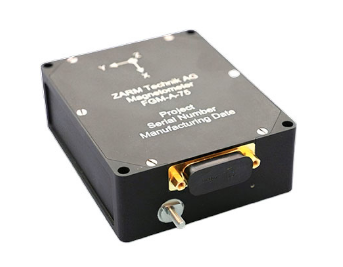
\includegraphics[height=50mm]{Figures/Magnetometer}
  \end{center}
  \caption{Example Magnetometer \cite{qp34}}
\end{figure}
A rate gyroscope, commonly referred to as a rate gyro measures the
angular velocity also in the body frame $\hat{\omega}_{B/I}=[\hat{g}_x,\hat{g}_y,\hat{g}_z]^T$. 
\begin{figure}[H]
  \begin{center}
  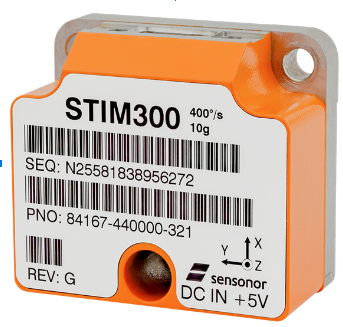
\includegraphics[height=50mm]{Figures/RateGyro}
  \end{center}
  \caption{Example IMU with Integrated Rate Gyro \cite{qp35}}
\end{figure}
Accelerometers are sensors used to measure acceleration at a point P
on a rigid body $\hat{a}_{B/I}=[\hat{a}_x,\hat{a}_y,\hat{a}_z]^T$. For simplicity however, it
is assumed that point P on the rigid body is the center of mass point
C therefore the accelerometer is measuring the acceleration of the
body itself in the body frame with respect to an inertial frame
$B/I$. 
\begin{figure}[H]
  \begin{center}
  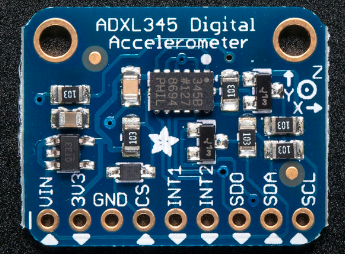
\includegraphics[height=50mm]{Figures/Accelerometer}
  \end{center}
  \caption{Example Accelerometer \cite{qp36}}
\end{figure}
As mentioned before, the IMU consists of 3 sensors all returning 3 measurments. This results in 9 scalar quantities being returned from this sensor which is where the term 9DOF gets it origin. In reality DOF means Degrees of Freedom which is contrary to the standard 6DOF simulation models explained above. However, the sensor community chooses to coin the term 9DOF to highlight the 9 different scalar values returned from IMUs. It is possible to obtain a 10DOF sensor which also returns pressure or temperature data. 

\subsubsection{Global Positioning System (GPS)}

The Global Positioning System (GPS) was developed in order to allow
accurate determination of geographical locations by military and civil
users. It works by using satellites in Earth’s orbit to transmit data
which makes it possible to measure the distance between the satellites
and the operator. This form of signal communication is incredibly
accurate and used heavily for attitude estimation. Up to 30 GPS
satellites are currently in orbit, mostly in MEO, at altitudes around
20,000 km. There will be between four and eight of them above any site
on the Earth at any time\cite{qp38}. These satellites continuously emit
coded high-frequency radio signals which may be received by special
GPS receivers. These signals contain information about the exact
orbits of the satellites and the time of atomic clocks onboard. When
signals from three or more satellites are received, the GPS receiver
will compute the best possible location of the user by
triangulation. Much like when on Earth, a GPS can be used for
navigation in space. The GPS receiver on board the satellite will also
receive its longitude, latitude, and altitude as long as it is within
the GPS constellation.
\begin{figure}[H]
  \begin{center}
  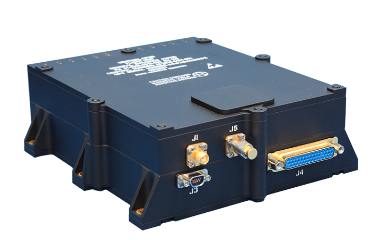
\includegraphics[height=50mm]{Figures/GPS}
  \end{center}
  \caption{Example GPS Receiver \cite{qp32}}
\end{figure}

\subsection{Euler Angle Estimation via IMU}

Using an IMU it is possible to obtain Euler Angles assuming a Flat Earth Approximation. Recall that Euler angles are a 3D transformation from the Inertial frame to the Body Frame (See Section \ref{s:Euler_Angles}). The angle $\phi$ and $\theta$ can directly be measured via the accelerometer by creating a relationship between the gravity vector in the inertial and body frames. The heading angle can be measured by creating a relationship between the magnetic field in the body frame and the inertial frame using a magnetometer. The rate gyro can be used to integrate the angular velocity to obtain Euler angles as well but is prone to drift. The accelerometer though is prone to errors when the vehicle experiences large acceleration loads. Thus, typically the Euler angles from the rate gyro are fused with the estimates from the magnetometer and the accelerometer. Still, some errors can still exist and the Euler angles can be fused with estimates from GPS but that will be explored in a separate section. First, let's examine the direct estimation of roll and pitch using the accelerometer. 

\subsubsection{Direct Measurement of Roll and Pitch}

Understand that the gravity vector in the inertial frame can be written as ${\bf C}_I(\vec{g}) = [0,0,g]^T$. However, since the first rotation in the Euler angle sequence is about the z-axis, the gravity vector in the A frame and Inertial (I) frames are identical. That is, ${\bf C}_A(\vec{g}) = {\bf C}_I(\vec{g})$. Normalizing the gravity vector yields ${\bf C}_A(\bar{g})=[0,0,1]^T$. The measurement from the accelerometer must also be normalized such that $\bar{a}_{B/I}=\hat{a}_{B/I}/||\hat{a}_{B/I}||$. Since the aircraft is always experiencing gravity, and the accelerometer is measuring the acceleration vector a relationship can be obtained between the gravity vector in the A frame and the acceleration vector in the body frame. Note that an assumption is being made here. It is assumed that the only acceleration being experienced is gravity. Therefore, if any external accelerations are experienced by the vehicle via thrust or aerodynamics, this equation is not valid. Still, for small UAV applications these equations can be accurate if fused properly with the rate gyro measurements. 
\begin{equation}
{\bf C}_B(\bar{a}_{B/I}) = {\bf T}_{NRB}^T{\bf T}_{ANR}^T{\bf C}_A(\bar{g}) = \begin{Bmatrix} -s_{\theta} \\ s_{\phi}c_{\theta} \\ c_{\phi}c_{\theta}\end{Bmatrix}
\end{equation}
The equation above takes the normalized gravity vector in the A frame and rotates it to the body frame through the no roll frame. Since the rotation is from the A frame to the body frame, only two rotations are required. Notice also that the first row can be used to obtain the pitch angle. 
\begin{equation}
\theta = -sin^{-1}(\bar{a}_x)
\end{equation}
The roll angle can then be obtained by taking the second two rows and dividing them together to get a tangent function. 
\begin{equation}
\phi = tan^{-1}\left(\frac{\bar{a}_y}{\bar{a}_z}\right)
\end{equation}
Note that this equation is only valid if $c_{\theta} \neq \pi/2$. This means the vehicle cannot fly straight up. For quadcopters and airplanes this is pretty typical for standard and level flight. For rockets however, either the IMU must be placed in an orientation that doesn't result in this singularity at launch or quaternions must be used. For spacecraft an entirely different algorithm is needed and is explained in a different section. 

Note that the pitch angle equation is written using the inverse sine function. Often times it is beneficial to compute the pitch angle using the inverse tangent function so that the {\it atan2} function may be utilized on a microcontroller which determines the quadrant of the angle more robustly. To do this the gravity vector must be written in the no roll frame. 
\begin{equation}
{\bf C}_{NR}(\bar{g}) = {\bf T}_{ANR}^T{\bf C}_A(\bar{g}) = \begin{Bmatrix} -s_{\theta} \\ 0 \\ c_{\theta}\end{Bmatrix}
\end{equation}
Then the acceleration vector is rotated to no roll frame as well from the body frame
\begin{equation}
{\bf C}_{NR}(\bar{a}_{B/I}) = {\bf T}_{NRB}{\bf C}_B(\bar{a}_{B/I}) = \begin{Bmatrix} \bar{a}_x \\ \bar{a}_y c_{\phi} - \bar{a}_z s_{\phi} \\ \bar{a}_y s_{\phi} + \bar{a}_z c_{\phi} \end{Bmatrix}
\end{equation}
Setting the two equations above equal to each other and diving the first row by the second row results in a tangent equation for pitch. This result is shown in the equation below.
\begin{equation}
\theta = -tan^{-1}\left(\frac{\bar{a}_x}{\bar{a}_y s_{\phi} + \bar{a}_z c_{\phi}}\right)
\end{equation}
Notice that these equations for pitch can be constructed by drawing a right triangle with the gravity vector as the hypotenuse. The sine function is the opposite side of the triangle divided by the hypotenuse which is 1 since the gravity vector was normalized while the inverse tangent function is the opposite side over the adjacent side. 

\subsubsection{Direct Measurement of Yaw}

In order to obtain the yaw angle of the vehicle through a direct measurement, the magnetometer is used. First it is assumed that the magnetic field strength is a constant through the flight of the vehicle and that it is oriented along the x-axis in the inertial frame of the Flat Earth Approximation. Remember that the x-axis is North using the Flat Earth Approximation. The magnetic field vector of the Earth is then normalized to unity. 
\begin{equation}
{\bf C}(\bar{\beta}_{\Earth}) = \begin{Bmatrix} 1 \\ 0 \\ 0 \end{Bmatrix}
\end{equation}
Again, in order to get a tangent function for the yaw angle estimation, the magnetic field of the Earth is written in the A frame. 
\begin{equation}
{\bf C}_A(\bar{\beta}_{\Earth}) = {\bf T}_{IA}^T{\bf C}_I(\bar{\beta}_{\Earth}) = \begin{Bmatrix} c_{\psi} \\ -s_{\psi} \\ 0 \end{Bmatrix}
\end{equation}
The magnetic field measurment of the magnetometer is then written in the A frame as well. However, the magnetometer measures the magnetic field in the body frame. Thus 2 rotations are requires to get from the body frame to the A frame. Again the magnetometer measurement is normalized.
\begin{equation}
{\bf C}_A(\bar{\beta}_{B}) = {\bf T}_{ANR}{\bf T}_{NRB}{\bf C}_B(\bar{\beta}_B)=\begin{Bmatrix} \bar{\beta}_x c_{\phi} + \bar{\beta}_y s_{\theta}s_{\phi} + \bar{\beta}_z c_{\phi}s_{\theta} \\ \bar{\beta}_y c_{\phi} - \bar{\beta}_z s_{\phi} \\ -\bar{\beta}_x s_{\theta} + \bar{\beta}_y s_{\phi}c_{\theta} + \bar{\beta}_z c_{\phi} c_{\theta} \end{Bmatrix}
\end{equation}
The two equations for magnetic field in the A frame can then be equated. In this case, the second row is divided by the first row to obtain a tangent relationship for yaw. The result for yaw is shown below.
\begin{equation}
\psi = tan^{-1}\left(\frac{\bar{\beta}_z s_{\phi} - \bar{\beta}_y c_{\phi}}{\bar{\beta}_x c_{\phi} + \bar{\beta}_y s_{\theta}s_{\phi} + \bar{\beta}_z c_{\phi}s_{\theta}}\right)
\end{equation}

\subsection{Low Earth Orbit Attitude Estimation}

In LEO the main algorithm begins with obtaining the magnetic field in
the body frame using magnetometers $\vec{\beta}_B$. Using the IGRF
model the locally measured magnetic field can be 
compared with the known magnetic field for any given location within
its orbit. Using the true data and the measured data, the spacecraft
can compute its actual position to the measured position and make the
correct adjustments. A Sun measurement is then taken using a Sun
sensor $\vec{S}_B$. Once those two independent 
body frame measurements are taken the inertial reference vectors must
be obtained from a database. Startrackers have this database built in;
however, for the magnetic field and the Sun vector these must be
obtained from a separate database as discussed in Section
\ref{s:ephemeris}. The idea is that if the position of the Earth is
known then the position of the Sun with respect to the Earth is also
known. The magnetic field vector can be 
obtained from the IGRF model as discussed in Section
\ref{s:magnetic_field}. The magnetic field vector in the inertial
frame is given as $\vec{\beta}_I$. Note that the IGRF model requires
the latitude and longitude to be known. Thus, in LEO a GPS is required
to feed into the database. The inertial Sun vector $\vec{S}_I$ only
requires the Julian time which can be obtained from GPS as well. The julian time is
based on the julian day as explained in Section \ref{s:ephemeris}.

The initial attitude determination algorithm itself requires two
independent vectors. As stated previously, startrackers provided a
large enough aperture and enough stars to produce the full
quaternion by obtaining multiple unique vectors to unique
stars. Multiple solar sensors or multiple magnetometers unfortunately
do not obtain non-unique vectors and the algorithm fails. In LEO this
is typically done with solar sensors and magnetometers but it can be
done with star trackers. In deep space it is typically done with
startrackers but it could be possible to obtain a Moon vector that
would require a Moon sensor.

The derivation below is done for the LEO case with a Sun and magnetic
field measurement. The derivation is identical for the deep space case
with a Moon sensor simply by substituting the magnetic field
measurment with a Moon measurement. Every vector is first normalized to obtain
$\hat{\beta}_B,\hat{\beta}_I,\hat{S}_B,\hat{S}_I$. A triad is then created
from body frame vectors using the equations below.
\begin{equation}
  \begin{matrix} \hat{f}_1 = \hat{S}_B & \hat{f}_2 = \hat{f}_1 \times
    \hat{\beta}_B & \hat{f}_3 = \hat{f}_1 \times \hat{f}_2 \end{matrix}
\end{equation}
The matrix ${\bf F}$ is then created using the triad as an orthonormal basis
$F = [\hat{f}_1,\hat{f}_2,\hat{f}_3]$. Similar equations are used for
the inertial measurements. 
\begin{equation}
  \begin{matrix} \hat{g}_1 = \hat{S}_I & \hat{g}_2 = \hat{g}_1 \times
    \hat{\beta}_I & \hat{g}_3 = \hat{g}_1 \times \hat{g}_2 \end{matrix}
\end{equation}
The matrix ${\bf G}$ is then created just as the ${\bf F}$ matrix such
that ${\bf G} =
[\hat{g}_1,\hat{g}_2,\hat{g}_3]$. The transformation from inertial to
body frame is then created using the formula below.
\begin{equation}
  {\bf T}_{BI} = {\bf FG}^T
\end{equation}
This matrix above is similar to the matrix in equation \ref{e:TIB} and
thus the Euler angles can be extracted from the matrix itself using
the formulation defined in Section \ref{s:Euler_Angles}. Euler can
then be converted to quaternions if needed. Note that it is relatively
easy to extract Euler angles from the ${\bf T}_{IB}$ matrix, it is not so
simple to extract quaternions. This is due to the fact that for every
orientation there exists two quaternions that represent this
space. Thus, it is more ideal to obtain Euler angles from the
transformation matrix and then convert them to quaternions.

\subsection{Spacecraft Position Estimation using a Ground Station Network (GSN)}

There are several types of ground stations depending on the
spacecraft’s distance from Earth. Ground services may be either
Direct-to-Earth (DTE) or space relay. DTE ground stations are located
on the Earth’s surface. They provide direct point-to-point access with
antennas at ground stations. DTE services are great for missions
needing frequent, short-duration contacts with high data transfer. 

Space relay services involve an intermediate satellite that
communicates with a ground station on the Earth’s surface. Relay
communication satellites for low-Earth orbit spacecraft can be in
Geosynchronous Equatorial Orbit (GEO), roughly 36,000 km from the
surface of Earth, or in low-Earth orbit. Relays are important for
providing communication and tracking when direct-to-ground
communications are not feasible due to physical asset visibility
constraints.  Space-based relay assets give missions full-time
coverage and continuous access to communication and tracking
services. 

Finally, deep space communication is also possible. The Deep Space
Network (DSN) is developed to conduct telecommunication and tracking
operations with space missions in GEO. This includes missions at lunar
distances, the Sun-Earth LaGrange points, and in highly elliptical
Earth orbits, and even missions to other planets\cite{qp40}. The DSN network
consists of three ground stations placed around 120 degrees apart on
Earth which provides 360 degrees coverage\cite{qp41}.
\begin{figure}[H]
  \begin{center}
  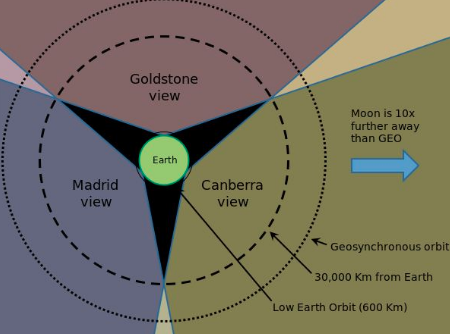
\includegraphics[height=80mm]{Figures/DSNSC}
  \end{center}
  \caption{Deep Space Network Satellite Coverage \cite{qp42}}
\end{figure}

\subsection{Heading Angle and Speed Estimation using GPS}

On Earth there is no need for a DSN because the vehicle is within the GPS constellation. Assuming the vehicle has the necessary GPS sensors a full NMEA (National Marine Electronics Association) can be obtained. However, in this example it is assumed that only the latitude, longitude and altitude coordinates are obtained in a discrete fashion. In order to get heading and speed it is assumed that consecutive measurements are obtained at $i$ and $i+1$ timestamps. Let's assume that the vehicle is traveling in a specific direction or heading and obtains a GPS coordinate $(\lambda_{LAT,i},\lambda_{LON,i},h_i)$ at time $t_i$. A few seconds later or whenever the update period may be the vehicle moves and the GPS returns a new GPS coordinate $(\lambda_{LAT,i+1},\lambda_{LON,i+1},h_{i+1})$ at time $t_{i+1}$. First, the coordinates are converted to a cartesian coordinate system. This is explained in the External Model section. This results in $x_i,y_i,z_i$ at time $t_i$ and $x_{i+1},y_{i+1},z_{i+1}$ at time $t_{i+1}$. First, the speed estimate is given by using a simple first order differentiation as given by
\begin{equation}
\begin{matrix}
v_x = (x_{i+1}-x_{i})/\Delta t \\
v_y = (y_{i+1}-y_{i})/\Delta t \\
\end{matrix}
\end{equation}
where $\Delta t = t_{i+1}-t_i$. Note that it is not recomended to compute the velocity in the z-axis as the altitude estimate of GPS is often not very good. Finally, the estimate for heading can follow from the speed estimate and is given as
\begin{equation}
\psi = tan^{-1}\left(\frac{v_y}{v_x}\right)
\end{equation}
Note that it is recommended to filter these estimates as GPS on its own is only accurate to around 3 meters.

\subsection{Spacecraft Attitude Control Schemes}

Many control schemes are needed to orient a satellite and all depend
on the application. In LEO magnetorquers can be used to detumble a
satellite while thrusters must be used in deep space. In addition
reaction wheels can be used to detumble a satellite anywhere in space
provided the angular momentum in the satellite does not saturate the
reaction wheels. Sections that follow detail the control schemes
typically utilized on small sats. A section on PID control for
aircraft is also in this section.

\subsubsection{B-dot Controller}

In LEO, the standard B-dot controller reported in many sources
(\cite{Leomanni2012},\cite{Lovera2015},\cite{WInstitute},\cite{SanyalDick})
can be used to de-tumble a satellite. The standard B-dot controller
requires the magnetorquers to follow the control law shown below
\begin{equation}\label{e:bdotcompact}
  \vec{\mu}_B = k{\bf S}(\vec{\omega}_{B/I}){\bf T}_{BI}(\vec{q})\vec{\beta}_I
\end{equation}
where $k$ is the control gain. Using equation (\ref{e:magmoment}) it
is possible to write the current in component form again
using the identity that $\vec{a}\times\vec{b}=-\vec{b}\times\vec{a}$
\begin{equation}\label{e:bdot}
  \begin{Bmatrix} i_{x}
    \\ i_{y} \\ i_{z} \end{Bmatrix} = \frac{k}{nA}\begin{bmatrix} 0 & \beta_z & -\beta_y \\ -\beta_z & 0 &
  \beta_x \\ \beta_y & -\beta_x & 0 \end{bmatrix}\begin{Bmatrix} p
    \\ q \\ r \end{Bmatrix}
\end{equation}
This equation can then be substituted into equation
(\ref{e:magtorquecomponent}) to produce the total torque on the
satellite assuming that the magnetorquers can provide the necessary
current commanded by equation (\ref{e:bdot}).
\begin{equation}\label{e:bdotfinal}
  \begin{Bmatrix} L \\ M \\ N \end{Bmatrix} = -k \begin{bmatrix}
    \beta_y^2 + \beta_z^2 & -\beta_x\beta_y & -\beta_x\beta_z
    \\ -\beta_x\beta_y & \beta_x^2 + \beta_z^2 & -\beta_y\beta_z \\
    -\beta_x\beta_z & -\beta_y\beta_z & \beta_x^2 +
    \beta_y^2 \end{bmatrix} \begin{Bmatrix} p
    \\ q \\ r \end{Bmatrix} 
\end{equation}
The goal of the controller here is to drive
$\vec{\omega}_{B/I}\rightarrow 0$. The literature will show that
this is not completely achieved \cite{Celani}. There are multiple
explanations for this. For starters, equation (\ref{e:magtorque})
assumes that the magnetic moment is not co-linear with the magnetic
field of the Earth. If it is, the result is zero torque applied to the
satellite. Furthermore, equation (\ref{e:bdot})
results in zero current if the angular velocity vector of the
satellite is co-linear with the magnetic field. Thus, if the magnetic
field vector, angular velocity vector or the magnetic moment vector
are co-linear, the torque applied to the satellite will be zero. If a
new operator is defined such that
\begin{equation}
  {\bf W}({\bf T}_{BI}(\vec{q})\vec{\beta}_I) = \begin{bmatrix}
    \beta_y^2 + \beta_z^2 & -\beta_x\beta_y & -\beta_x\beta_z
    \\ -\beta_x\beta_y & \beta_x^2 + \beta_z^2 & -\beta_y\beta_z \\
    -\beta_x\beta_z & -\beta_y\beta_z & \beta_x^2 +
    \beta_y^2 \end{bmatrix}
\end{equation}
it is easy to see that the torque applied to a satellite is then
simply the angular velocity vector multiplied by this transition
matrix. If this transition matrix is put into row-reduced-echelon form
it is easy to see that the determinant of this matrix is equal to
zero (\cite{carlen2006linear}).
\begin{equation}
  rref({\bf W}({\bf T}_{BI}(\vec{q})\vec{\beta}_I) = \begin{bmatrix} 1 & 0
    & -\beta_x/ \beta_z \\ 0 & 1 & -\beta_y/ \beta_z \\ 0 & 0 & 0 \end{bmatrix}
\end{equation}
A zero determinant means that there exists a vector
$\vec{\omega}_{B/I}$ that will result in zero torque for a given value
of the magnetic field. This is typically avoided since the
magnetic field of the Earth is time and spatially varying
which results in a transition matrix that changes over time due to
orientation changes in the satellite as well as changes in the satellite's
orbit. However, for low inclination orbits, it's possible for the
magnetic field to stay relatively constant with $\beta_x \approx
\beta_y \approx 0$. If the satellite is tumbling about the yaw axis such
that $p=q=0$, the yaw torque on the satellite ($N$) will be
zero. Using this simple controller, there is no way to
remove the remaining angular velocity from the satellite unless
reaction wheels are used.

\subsubsection{Reaction Wheel Control}

Assuming each reaction is aligned with a principal axis of inertia the
control scheme is extremely simple. When the wheels are not aligned
the derivation will proceed similar to the reaction control thruster
section. The derivation here will just be for the aligned case. In
this analysis it is assumed that a torque can be applied to the
reaction wheel and thus the angular velocity of the reaction wheel
$\alpha_{Ri}$ can be directly controlled. Assuming this a simple PD
control law can be used to orient the satellite at any desired
orientation using Euler angles for this control law since the
satellites are aligned with the principal axes of rotation \cite{etkins}.
\begin{equation}
  \alpha_{Ri} = -k_p(\epsilon_i-\epsilon_{desired})-k_d(\omega_i-\omega_{desired})
\end{equation}
In the equation above $\epsilon$ denotes either roll $\phi$, pitch
$\theta$ or yaw $\psi$ depending on which reaction wheel is being
used. The Euler angles in this case would be obtained by converting
the quaternions to Euler angles as defined in Section \ref{s:quat}.

Often times however your reaction wheels are not pointed on the
principal axis of inertia. In this case a Least Squares Regression
model is needed. In this case the equation above is used to compute
the desired torque to be placed on the satellite such that
\begin{equation}
  \vec{M}_{desired} = -k_p(\epsilon_i-\epsilon_{desired})-k_d(\omega_i-\omega_{desired})
\end{equation}
This equation is then equated to the equation for torque placed on the
satellite where the angular accelerations are placed into a vector.
\begin{equation}
  \vec{M}_{desired} = \vec{M}_R = \sum\limits_{i=1}^{NR}
  I^{B}_{Ri}\alpha_{Ri}\hat{n}_{Ri} = \begin{bmatrix}
    I^{B}_{R1}\hat{n}_{R1} & \hdots &
    I^{B}_{RNR}\hat{n}_{RNR} \end{bmatrix} \begin{Bmatrix} \alpha_1
    \\ \vdots \\ \alpha_{NR} \end{Bmatrix} = {\bf J} \vec{\alpha}
\end{equation}
Since ${\bf J}$ is a $3\times{N_{RW}}$ matrix its impossible to simply
invert the matrix and solve for the vector of angular accelerations
$\vec{\alpha}$. In this case there are an infinite number of
solutions. As such a minimization routine is required where the
solution found also happens to be the lowest amount of angular
acceleration. In this case, Lagrange's method was used to find the
vector of angular accelerations \cite{lagrange}.
\begin{equation}
  \vec{\alpha} = {\bf J}^T\left({\bf J}{\bf J}^T\right)^{-1}\vec{M}_{desired}
\end{equation}

\subsubsection{Reaction Control Thrusters}

The control law for the thrusters is a bit complex if the location of
thrusters is not know apriori. If the location {\it is} known then
simple PID control laws can be generated by applying pure couples to
the correct thrusters that activate the correct axes. If the location
{\it is not} known then the following derivation will suffice. There
are $N_P$ thrusters and only 3 degrees of freedom that need to be
controlled; thus, the system is an overactuated system. Using equation
\ref{e:propulsion}, the equation can be written in matrix form as
given by the equation below where $\vec{M}_p$ is replaced by
$\vec{M}_{desired}$. The equation for $\vec{M}_{desired}$ is generated
using a similar PD control law as the reaction wheels. 
\begin{equation}
  \vec{M}_{desired} = p[{\bf S}(\vec{r}_{P1})\hat{n}_{P1}~~{\bf
      S}(\vec{r}_{P2})\hat{n}_{P2}~~\hdots~~{\bf
      S}(\vec{r}_{P{N_p}})\hat{n}_{P{N_p}}]\vec{\sigma} = {\bf M}\vec{\sigma}
\end{equation}
Since ${\bf M}$ is a $3\times{N_P}$ matrix its impossible to simply
invert the matrix and solve for the vector of pulses
$\vec{\sigma}$. In this case there are an infinite number of
solutions. As such a minimization routine is required where the
solution found also happens to be the least amount of pulses. In this
case, Lagrange's method was used to find the vector of pulses \cite{lagrange}.
\begin{equation}
  \vec{\sigma} = {\bf M}^T\left({\bf M}{\bf M}^T\right)^{-1}\vec{M}_{desired}
\end{equation}
Note that a similar equation can be derived for
$\vec{F}_{desired}$. The solution to the equation above results in
values of $\sigma$ that are bigger than 1 and sometimes negative. If a
value in this vector is bigger than 0 the value is set to 1 and
if the value is negative the value is set to 0. Thus, the solution
does not yield an exact solution but it does allow for flexibility in
the number of thrusters and their respective orientations. Sizing of
the thrusters depends on many independent variables 
including the thrust $T$ and the $I_{sp}$. Using the $I_{sp}$ the exit
velocity of the thruster can be obtained by using the equation below
\begin{equation}
  v_e = I_{sp}g_0
\end{equation}
where $g_0$ is the gravitational acceleration of the Earth at
sea-level. Then the mass flow rate of the thruster can be obtained
using the equation below.
\begin{equation}
  \dot{m}_P = T/v_e
\end{equation}
Using this mass flow rate total propellant mass required can be
computed assuming a certain duty cycle.

\subsubsection{Cross Products of Inertia Control}

An interesting form of control is to take advantage of momentum
dumping. Looking at the equation for angular acceleration again (Eqn \ref{e:pqrdot}) this
equation can be simplified for certain cases. For example, if the roll
rate of the satellite is set to be non-zero while the pitch rate and
yaw rates are set to zero it is easy to see that if the inertia is
diagonal the derivative of angular velocity is zero. However, if the
cross products of inertia are given by the matrix below
\begin{equation}
  {\bf I}_s = \begin{bmatrix} I_{xx} & I_{xy} & I_{xz} \\ I_{xy} &
    I_{yy} & I_{yz} \\ I_{xz} & I_{yz} & I_{zz} \end{bmatrix}
\end{equation}
the derivative of angular velocity becomes
\begin{equation}
  \dot{\vec{\omega}}_{B/I} = I_S^{-1} \left (\begin{Bmatrix} 0
    \\ -I_{xz}p^2 \\ I_{xy}p^2 \end{Bmatrix} \right )
\end{equation}
again assuming the roll rate is non zero and the pitch rate is
zero. This result shows that momentum can be transferred to different
axes provided the cross products of inertia are non-zero.

\subsection{PID Control of a Fixed Wing Aircraft}

For a conventional PID controller of an aircraft, the rudder, elevator
and aileron commands are set to 
\begin{equation}
\begin{matrix}
\delta_{r} =-K_v v \\
\delta_{e} = K_p(\theta-\theta_{c})+K_d{\dot \theta} \\ 
\delta_a = K_p(\phi-\phi_{c})+K_d{\dot \phi}
\end{matrix}
\end{equation}
The Euler angle commands $\phi_{c}$ and $\theta_{c}$ are set using the
following relationships:
\begin{equation}
  \begin{matrix}
  \phi_{c} = K_p(\psi-\psi_c)+K_d\dot{\psi} \\
  \theta_{c} = K_p(z-z_c) + K_d\dot{z} + K_{I}\int{z-z_c}dt
  \end{matrix}
\end{equation}
The control scheme defined above is a conventional inner loop-outer
loop control of a fixed wing aircraft using a PID tracking
controller.

\subsection{Controllability}

Controllability is formally stated as a system where any initial
state $x(0)=x_0$ and final state $x_1,t_1>0$, there exists a piecewise
continuous input $u(t)$ such that $x(t_1)=x_1$. 
For a fixed wing aircraft the system has 12 states with 8 dynamic
modes and 4 zero or rigid body modes. For a fixed wing aircraft the system has 12 states with 8 dynamic
modes and 4 zero or rigid body modes. A conventional aircraft has 4
controls to control these 12 modes. The easiest way to test the 
controllability of a system  is to compute the
controllability matrix. However, the controllability matrix must be
computed using a linearized model such that
$\dot{\vec{x}}=A\vec{x}+B\vec{u}$. In order to do this the aircraft
must be in equilibrium. For this example the aircraft is
set with an initial velocity of $20~m/s$ at an altitude of
$200~m$. The altitude command is set to $200~m$ and the heading
command is set to zero. Given the zero heading angle command and the
symmetry of the configurations investigated the rudder and aileron
commands are set to zero. Thus, only the thrust and elevator controls
are activated for the trimming procedure. Each configuration is
simulated for 200 seconds or until the derivatives of all states
except $\dot{x}$ are within a required tolerance. Using this
equilibrium point a linear model can be computed by using forward
finite differencing assuming that the
aircraft model is put in the form $\dot{\vec{x}} = F(\vec{x},\vec{u})$.
\begin{equation}
\dot{\vec{\delta x}} = \frac{F(\vec{x_0}+\Delta \vec{x_0},\vec{u_0})-F(\vec{x_0},\vec{u_0})}{\Delta
  \vec{x}}\vec{\delta x} + \frac{F(\vec{x_0},\vec{u_0}+\Delta
  \vec{u})-F(\vec{x_0},\vec{u_0})}{\Delta \vec{u}}\vec{\delta u}
\end{equation}
This linear model is the classic linear model where
$\dot{\vec{\delta x}}=A\vec{\delta{x}}+B\vec{\delta{u}}$. Using this linear model, the
controllability matrix can be computed as
\begin{equation}
W_C = [B~AB~A^2B~A^3B~...~A^{N-1}B]
\end{equation}
where N is the number of states in the system. With the controllability
matrix formulated, the rank of the matrix is computed. If the
$rank(W_C)=N$ the system is said to be controllable.
